\RequirePackage{plautopatch}
\documentclass[upLaTeX,a4paper]{jsarticle}
\usepackage{listings,jlisting,amsmath,otf}
\usepackage[dvipdfmx]{graphicx}

\lstset{
breaklines = true,
numbers = left,
frame = tbrl,
tabsize = 4,
captionpos = t
}

\title{流体の数値計算プログラムの作成 中間報告}
\author{B4 津田修一朗}
\date{}

\begin{document}
\maketitle

\section{これまでに取り組んだこと}
\subsection{環境構築}
gfortranとgnuplotをインストールした.
エディタはVisual Studio Codeを使用している.

\subsection{流れ関数と渦度を求めるプログラムの実装}
流れ関数-渦度法により,cavity内の流れを解いた.基礎方程式については,資料「流体の数値計算(川口光年先生1976年頃).pdf」に従った.

\section{速度ベクトルの図の描画}
流れ関数と渦度を求めるプログラムの実装により得られた流れ関数$\phi$より,速度場$(u, v)$を

\begin{equation}
  u = \frac{\partial \phi}{\partial y}, v = - \frac{\partial \phi}{\partial x},
\end{equation}
を用いて求めた.

図1は
\begin{figure}[htbp]
  \begin{center}
    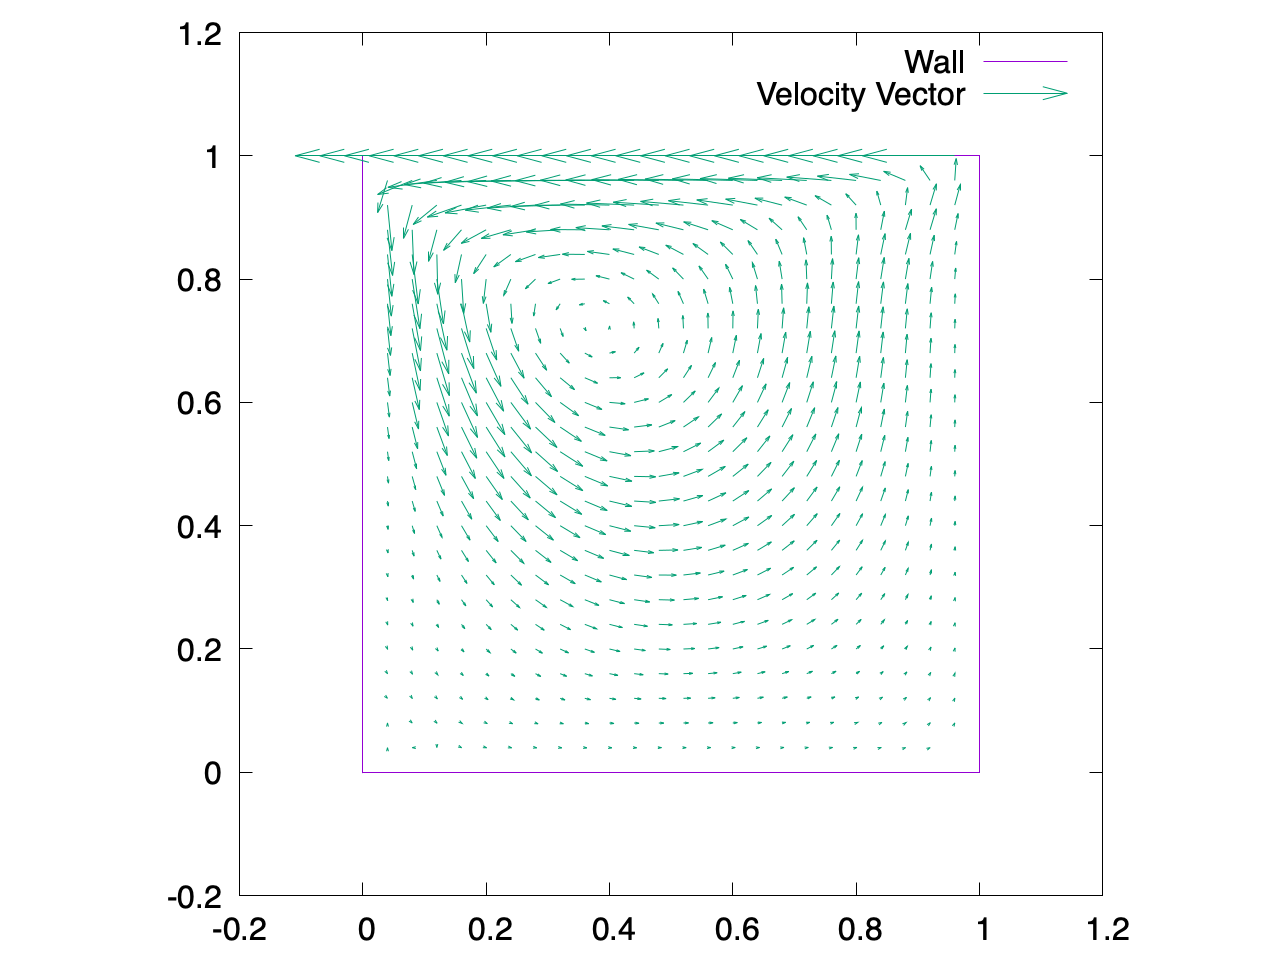
\includegraphics[width=15cm]{outputs/img/velocity_vector.png}
  \end{center}
  \caption{タイトル}
  \label{picture}
\end{figure}
\end{document}